\documentclass[11pt]{article}
\usepackage[margin=1in]{geometry}
\usepackage{graphicx}
\graphicspath{{figs/}}
\usepackage{amsmath,amssymb,amsthm,booktabs,float}
\usepackage[hidelinks]{hyperref}

\newtheorem{theorem}{Theorem}
\newtheorem{lemma}{Lemma}
\newtheorem{proposition}{Proposition}
\newtheorem{corollary}{Corollary}
\theoremstyle{definition}
\newtheorem{definition}{Definition}

\newcommand{\R}{\mathbb{R}}
\newcommand{\E}{\mathbb{E}}
\newcommand{\Prob}{\mathbb{P}}
\newcommand{\one}{\mathbf{1}}
\newcommand{\rank}{\operatorname{rank}}
\newcommand{\diag}{\operatorname{diag}}
\newcommand{\tr}{\operatorname{tr}}
\newcommand{\RP}{\mathbb{R}\mathrm{P}}
\DeclareMathOperator*{\argmin}{arg\,min}
\DeclareMathOperator*{\argmax}{arg\,max}

\title{What Is a Brain State? Rank-2 Phase Dynamics, J-Space Occupancy Degeneracy,\\
and a Pattern-Defined ADHD Effect}
\author{Felicity Li \and Quhao Chen}
\date{}

\begin{document}
\maketitle

\begin{abstract}
We study two identifiability questions that arise when a high-dimensional time series is
summarized by clustering and by a fitted linear operator: when is a cluster label a
transferable coordinate rather than an arbitrary name, and when does the operator carry
information beyond the occupancy of the labels? We answer both for a phase-based model of
brain dynamics. First, the Leading Eigenvector Dynamics Analysis (LEiDA) phase-alignment
matrix is positive semidefinite of rank at most two, with closed-form eigenvalues and
leading eigenvector, and a $\mathbb{Z}_2$ sign gauge. Second, we define a custom
\emph{J-space} for a learned switching-linear latent field
$z_{t+1}=A(p_t)z_t+b(p_t)$, where $p_t$ is a one-hot LEiDA label and
$A(p)=\sum_s p_sA_s$. Because the field is linear in $z$ and the labels are one-hot, the
per-frame Jacobian is exactly $A(p_t)$; its stay-frame average
$\bar J=\sum_s f_sA_s$ lies in the convex hull of the shared operators and has at most
$k-1=2$ degrees of freedom. Every singular-value summary of $\bar J$ is therefore a
function of the occupancy $f$; the learned operator cannot supply independent dynamical
evidence beyond occupancy. We then prove that named $k$-means state indices are not
identifiable: under independent refits the expected index recovery is $1/k$, while the
pattern-matched effect can be stable. In ADHD-200 ($n=665$), the pattern-matched LEiDA
occupancy effect is negative and robust (ADHD lower occupancy; fixed-effect meta
$d=-0.302$, within-site-code permutation $p=0.001$ [2,000-draw floor], FWER $0.001$
[1,000-draw floor], split-half reliability $0.586$; motion-matched paired
$d_z\approx-0.17$, matched between-group $d\approx-0.25$, $p=0.006$), but the literal
named-index effect is null ($d=-0.035$), and 40 refits recover the index at chance
($22.5\%$ vs $20\%$). The $\bar J$ spectral metrics are occupancy functions and show
null group means. This is a single-cohort reanalysis: the $k=5$ sample overlaps the ADHD-200 sample of
de Lacy and Calhoun by $70.5\%$, and one site code reverses. We conclude that the ADHD
phase-state difference is real but pattern-defined in this cohort, and that named-state
claims in dynamic-FC analyses are not identifiable without a refit-identifiability test.
\end{abstract}

\section{Introduction}

A high-dimensional time series is often summarized by partitioning its frames into a
small number of groups. The partition induces labels $\ell(t)\in\{1,\dots,k\}$ and
occupancies $\pi_s$, but the labels are not part of the data: permuting the group names
leaves the partition unchanged while changing every statement about ``state $s$.''
Whether a named index can be recovered from an independent fit is an identifiability
question. In mixture models it is the label-switching problem
\cite{Stephens2000,Jasra2005}; in cluster analysis it is the stability problem
\cite{Hennig2007,vonLuxburg2010}. In the dynamic-state literature it is often left
implicit: states are reported by index, as if the integer were a coordinate.

A second question appears when a dynamical model is fitted to the same labels. Consider
the switching-linear field
\begin{equation}
z(t+1)=A(p_t)z(t)+b(p_t),
\qquad
A(p)=\sum_{s=1}^{k}p_sA_s,
\end{equation}
where $p_t$ is the one-hot encoding of $\ell(t)$ and the operators $A_s$ are shared
across subjects. The per-frame Jacobian is exactly $J(t)=A(p_t)$. Over the stay frames
of a subject, the average is a convex combination,
\begin{equation}
\bar J=\frac1n\sum_{t\in\mathrm{stay}}J(t)
=\sum_{s=1}^{k}f_sA_s,
\qquad
f_s=\frac{n_s}{n},
\qquad
\sum_s f_s=1,
\end{equation}
where $n_s$ is the number of stay frames in state $s$. Every scalar summary of $\bar J$
is then a function of the occupancy $f$: the operator cannot supply independent evidence
about dynamics beyond occupancy. This is a fact about shared-operator switching-linear
models, not about a particular dataset, and it is the second theme of the paper.
At each level of a dynamic-state claim---the matrix, the operator, the index---we ask
what is identifiable, and what survives.

We study these questions in a phase-based model of resting-state functional magnetic
resonance imaging (fMRI). Blood-oxygen-level-dependent (BOLD) signals from $N$ brain
parcels are band-pass filtered and z-scored; the Hilbert transform gives an instantaneous
phase $\phi_i(t)$ for each parcel. The instantaneous phase-alignment (iPA) matrix is
\begin{equation}
C_{ij}(t)=\cos\big(\phi_i(t)-\phi_j(t)\big).
\end{equation}
Leading Eigenvector Dynamics Analysis (LEiDA) takes the leading eigenvector $v_1(t)$ of
$C(t)$ and clusters the time series $\{v_1(t)\}$ into $k$ states
\cite{Cabral2017,Glerean2012,Tang2026}. Occupancy, lifetime, and switching of these
states are the standard summaries, and group differences in state occupancy have been
reported in attention-deficit/hyperactivity disorder (ADHD) and other conditions
\cite{deLacy2019,Shappell2021,Ahmadi2021,Kaboodvand2020}. Those claims are keyed to an
integer state index, which is exactly the first question.

On the operator side, we fit a switching-linear latent model
\cite{Linderman2017,Taghia2018,Chen2018} to the same leading eigenvectors. For each
subject we compute the average Jacobian $\bar J$ over stay frames, decompose it by
singular value decomposition $\bar J=U\Sigma V^{\top}$, and summarize its spectral
geometry by the concentration $C_k$ and the effective rank $r_{\mathrm{eff}}$. We call this derived
object---the SVD geometry of the average Jacobian, together with its scalar
summaries---the \emph{J-space} of the subject. We use this term for the derived object;
it is built on top of the LEiDA state. It is the quantity a learned-dynamics analysis
would ordinarily treat as a dynamical phenotype.

The mathematics of the iPA matrix sharpens the first question. The matrix is rank 2, but
its leading eigenvector is an $N$-vector: rank 2 is a statement about the spectral
subspace, not about the state. The eigenvector is defined only up to sign, and a change
of sign convention changes the label sequence; a substantial fraction of apparent state
transitions is gauge drift rather than dynamics. The J-space has a second degeneracy.
With $k$ shared operators, $\bar J$ lies in a $(k-1)$-simplex, so the two-number object
is the occupancy, not the operator. These are the structural results of Sections
\ref{sec:leida} and \ref{sec:jspace}.

\subsection*{Hypotheses}

We make two predictions. First, the iPA matrix is rank 2, so the identity holds frame
by frame and every $\bar J$ spectral metric is predictable from occupancy, with no
metric surviving occupancy control. Second, ADHD differs in pattern-matched
occupancy but not in a named index: the pattern effect is negative under a
within-site permutation null with adequate reliability, the literal effect is null,
and refits recover the index near the $1/k$ chance level.

Results follow this structure. The rank-2 identities hold to machine precision; the
$\bar J$ spectral metrics are occupancy-dominated (linear $R^2$ $0.56$--$0.66$,
quadratic $0.73$--$0.77$), their group means are null, and the coupling between the
J-space metrics and an independent $k=5$ occupancy lens collapses after occupancy
control. In that $k=5$
lens ($n=665$), the pattern-matched occupancy effect is negative and robust:
$d=-0.302$, within-site-code permutation $p=0.001$ (2,000-draw floor), FWER $0.001$
(1,000-draw floor), split-half reliability $0.586$; motion-matched paired
$d_z\approx-0.17$ (between-group $d\approx-0.25$), $p=0.006$. The literal index effect is null
($d=-0.035$), and $40$ refits recover the index at $22.5\%$ versus $20\%$ chance; the
pattern-matched effect is $-0.299$ with all refits negative. The effect is
pattern-defined, not index-defined. The $k=5$ cohort overlaps the ADHD-200 sample of
de Lacy and Calhoun \cite{deLacy2019} by $469/665$ ($70.5\%$; their Supplementary
Table S3), so this is a reanalysis rather than an independent-cohort replication; we
return to this in the constraints.

The rank-2 decomposition and the sign ambiguity are not new
\cite{Glerean2012,Olsen2022,EiDA2024}, and the switching-linear model class is standard
\cite{Linderman2017,Taghia2018}. What is new is the J-space construction and the
identification of its stay-field summaries as occupancy functions, the identifiability
result for named states with its $1/k$ baseline, and the pattern-defined negative
difference with the index claim removed. The paper's claim is not that the brain has a
two-dimensional state. It is that rank 2 is a statement about a spectral subspace, that
the J-space is a two-degree-of-freedom occupancy in disguise, that a named cluster index
is not a coordinate, and that the ADHD occupancy difference is real when it is
pattern-defined.

The mathematical core is in Sections \ref{sec:leida}--\ref{sec:identifiability}; the
data and results are in Sections \ref{sec:methods}--\ref{sec:results}.

\section{Phase Alignment and LEiDA}
\label{sec:leida}

\subsection{Phase extraction}
Let $x_i(t)$ be the BOLD signal of parcel $i\in\{1,\dots,N\}$ at frame
$t\in\{1,\dots,T\}$. After band-pass filtering and z-scoring, form the analytic signal
\begin{equation}
x_i(t)+i\,\mathcal{H}[x_i](t)=A_i(t)e^{i\phi_i(t)},
\end{equation}
where $\mathcal{H}$ is the Hilbert transform and $\phi_i(t)\in[0,2\pi)$ is the
instantaneous phase. Write $c_i(t)=\cos\phi_i(t)$ and $s_i(t)=\sin\phi_i(t)$.

\subsection{The instantaneous phase-alignment matrix}
The iPA matrix is
\begin{equation}
C_{ij}(t)=\cos\!\big(\phi_i(t)-\phi_j(t)\big)
=c_i(t)c_j(t)+s_i(t)s_j(t),
\end{equation}
or, in matrix form,
\begin{equation}
C(t)=c(t)c(t)^{\top}+s(t)s(t)^{\top}.
\label{eq:Crank}
\end{equation}
$C(t)$ is symmetric, positive semidefinite, has unit diagonal, and $\tr C(t)=N$.

\begin{theorem}[Rank-2 phase alignment]
\label{thm:rank2}
For every $t$, $\rank C(t)\le 2$. Let
$\sum_{j=1}^N e^{2i\phi_j(t)}=A(t)e^{2i\psi(t)}$ with $A(t)\ge0$ and
$\psi(t)\in[0,\pi)$, and define $R_2(t)=A(t)/N\in[0,1]$. Then the non-zero eigenvalues
of $C(t)$ are
\begin{equation}
\lambda_1(t)=\frac{N+A(t)}{2}=\frac{N}{2}\big(1+R_2(t)\big),
\qquad
\lambda_2(t)=\frac{N-A(t)}{2}=\frac{N}{2}\big(1-R_2(t)\big),
\end{equation}
with orthonormal eigenvector
\begin{equation}
v_1(t)=\frac{\cos(\phi(t)-\psi(t))}{\sqrt{\lambda_1(t)}},
\end{equation}
where the cosine and sine are applied elementwise. In particular,
\begin{equation}
\frac{\lambda_1(t)}{N}=\frac{1+R_2(t)}{2}\ge\frac12.
\label{eq:l1identity}
\end{equation}
\end{theorem}

\begin{proof}
Equation \eqref{eq:Crank} gives $\rank C\le2$ and positive semidefiniteness. The
non-zero spectrum of $C$ equals the spectrum of the $2\times2$ Gram matrix
\begin{equation}
G=\begin{pmatrix}c^{\top}c & c^{\top}s\\ s^{\top}c & s^{\top}s\end{pmatrix}.
\end{equation}
Write $\sum_j e^{2i\phi_j}=A e^{2i\psi}$. Then
\begin{equation}
c^{\top}c=\frac{N+A\cos2\psi}{2},\quad
s^{\top}s=\frac{N-A\cos2\psi}{2},\quad
c^{\top}s=\frac{A\sin2\psi}{2}.
\end{equation}
The eigenvalues of $G$ are $(N\pm A)/2$, with eigenvectors
$(\cos\psi,\sin\psi)^{\top}$ and $(-\sin\psi,\cos\psi)^{\top}$. Mapping back to $\R^N$
gives $v_1\propto c\cos\psi+s\sin\psi=\cos(\phi-\psi)$ and
$v_2\propto-c\sin\psi+s\cos\psi=\sin(\phi-\psi)$; normalizing with $\lambda_1,\lambda_2$
gives the stated forms. Finally $\lambda_1+\lambda_2=N$ and
$\lambda_1/N=(1+R_2)/2$.
\end{proof}

\begin{corollary}[The leading eigenvector is an $N$-vector, not a two-number state]
\label{cor:not2d}
The matrix $C(t)$ has a two-dimensional \emph{spectral subspace}, but the leading
eigenvector $v_1(t)\in\R^N$ is an $N$-dimensional object. The pair $(\psi(t),R_2(t))$ is
a two-parameter summary of the phase configuration, not a lossless encoding of
$v_1(t)$: the full phase vector $\phi(t)$ is required to reconstruct $v_1(t)$.
\end{corollary}

\begin{proof}
Immediate from Theorem \ref{thm:rank2}:
$v_1(t)=\cos(\phi(t)-\psi(t))/\sqrt{\lambda_1(t)}$ depends on the whole vector $\phi(t)$
through the elementwise cosine. The pair $(\psi,R_2)$ determines only the mean phase and
the coherence magnitude, i.e.\ two summary statistics.
\end{proof}

Corollary \ref{cor:not2d} is worth stating explicitly: the phrase ``the state is
two-dimensional'' is not justified for the leading eigenvector. What is
two-dimensional is the spectral subspace of $C(t)$ (rank 2) and, separately, the
occupancy simplex of the J-space in Section \ref{sec:jspace}. The empirical state in
LEiDA is the projective class $[v_1(t)]\in\RP^{N-1}$; clustering acts on that projective
space, not on a two-dimensional parameter space.

\subsection{Sign gauge}
The eigenvector equation determines $v_1(t)$ only up to sign: $v_1(t)$ and $-v_1(t)$ are
the same projective point, and $C(t)$ is invariant. A \emph{gauge} is a choice of
representative $\pm v_1(t)$ at each frame.

\begin{lemma}[$\mathbb{Z}_2$ gauge]
\label{lem:gauge}
Let $g(t)\in\{\pm1\}$ be a gauge field and let $\tilde v_1(t)=g(t)v_1(t)$. Then $C(t)$
is unchanged, but the label sequence
$\ell(t)=\argmin_j\|v_1(t)-\mu_j\|$ and the transition matrix
$P_{ij}=\Prob(\ell(t+1)=j\mid\ell(t)=i)$ depend on $g$. Consequently any statistic of
$\ell$ or $P$ is gauge-dependent unless it is defined on the projective class $[v_1]$.
\end{lemma}

\begin{proof}
$C$ is homogeneous of degree zero in the sign of its eigenvectors. The nearest-centroid
rule is not invariant if the centroids are fitted in a signed representation: flipping a
subset of frames moves those frames to the antipodal side of the sphere, changing
assignments. The transition matrix is a function of the label sequence, hence changes
with $g$. A statistic defined on $[v_1]$ is invariant by construction.
\end{proof}

In practice the gauge is fixed by a convention (majority-positive, majority-negative,
max-absolute-component-positive, or continuity-aligned). These conventions disagree on a
substantial fraction of frames; in an HBN resting-state sample of $180$ subjects, the
max-component convention flipped on $32.3\%$ of frames and the majority-negative
convention on $11.3\%$. When the max-component gauge flipped, a label switch followed
with probability $0.822$, versus $0.124$ when it did not; under the majority-negative
gauge the corresponding probabilities were $0.311$ and $0.063$. A large fraction of
``state transitions'' is therefore gauge drift, and the label sequence is not
gauge-invariant unless the clustering is performed projectively. In the analysis below
we fix the max-absolute-component gauge for the $k=5$ lens and use the majority-negative
gauge for the $k=3$ J-space lens; the rank-2 and occupancy theorems are
gauge-independent, while the named labels are not.

\subsection{Clustering and named states}
LEiDA clusters the time series of $[v_1(t)]$ into $k$ centroids
$\mu_1,\dots,\mu_k$ by $k$-means and assigns
$\ell(t)=\argmin_j d([v_1(t)],[\mu_j])$. The occupancy of state $s$ is
\begin{equation}
\pi_s=\frac1T\sum_{t=1}^{T}\one[\ell(t)=s].
\end{equation}
The index $s$ is a bookkeeping device: a permutation of the centroids leaves the
partition unchanged but changes every statement about ``state $s$.'' Whether a named
index is recoverable across independent fits is the identifiability question of Section
\ref{sec:identifiability}.

The pair $(\psi,R_2)$ above---mean phase and coherence---is a two-parameter projection
of $\phi(t)$, not the leading eigenvector itself.

\section{The J-Space: Definition and Occupancy Degeneracy}
\label{sec:jspace}

The J-space is a derived object. It is built on top of the LEiDA label sequence and is
not assumed from prior literature; we define it here and use the name for the rest of
the paper.

\begin{definition}[J-space]
Let $v(t)\in\R^N$ be the leading eigenvector of the iPA matrix and
$\ell(t)\in\{1,\dots,k\}$ its LEiDA label. Let $z(t)\in\R^d$ be a latent state given
by a causal encoder $z(t)=E(v(t-w+1),\dots,v(t))$, and let
\begin{equation}
z(t+1)=A(p_t)z(t)+b(p_t),
\qquad
A(p)=\sum_{s=1}^{k}p_sA_s,
\qquad
b(p)=\sum_{s=1}^{k}p_sb_s,
\label{eq:field}
\end{equation}
with $p_t\in\{0,1\}^k$ the one-hot encoding of $\ell(t)$ and
$A_s\in\R^{d\times d}$, $b_s\in\R^d$ shared across subjects. The per-frame Jacobian is
\begin{equation}
J(t)=\frac{\partial z(t+1)}{\partial z(t)}=A(p_t).
\label{eq:Jt}
\end{equation}
For a subject, let
\begin{equation}
\bar J=\frac1n\sum_{t\in\mathrm{stay}}J(t)
=\sum_{s=1}^{k}f_sA_s,
\qquad
f_s=\frac{n_s}{n},
\qquad
\sum_s f_s=1,
\label{eq:Jbar}
\end{equation}
over the $n$ stay frames (frames with $\ell(t)=\ell(t+1)$ and
$\cos(v(t),v(t+1))\ge-0.5$), where $n_s$ is the number of stay frames in state $s$.
Write $\bar J=U\Sigma V^{\top}$ with singular values
$\sigma_1\ge\cdots\ge\sigma_d\ge0$, let $V_k=[v_1,\dots,v_k]$ be the leading right
singular vectors, and let $A_J=V_k^{\top}\bar J V_k$. The \emph{J-space} of the subject
is the tuple $(\bar J,U,\Sigma,V,V_k,A_J)$ together with the scalar summaries
\begin{equation}
C_k=\frac{\sum_{i=1}^{k}\sigma_i^2}{\sum_{i=1}^{d}\sigma_i^2},
\qquad
r_{\mathrm{eff}}=\frac{(\sum_i\sigma_i)^2}{\sum_i\sigma_i^2},
\end{equation}
\end{definition}

\begin{remark}[Occupancy degeneracy of the J-space]
\label{thm:occupancy}
For the field \eqref{eq:field} with shared operators $A_s$ and one-hot conditioning
$p_t$, $J(t)=A(p_t)$ is independent of $z(t)$, $\bar J=\sum_s f_s A_s$ lies in
$\mathrm{conv}\{A_s\}$ (affine dimension at most $k-1$), and every scalar function
$g(\bar J)$ is a function $h_g(f)$ with $\sum_s f_s=1$---in particular, with $k=3$,
every stay-field metric depends on at most two numbers.
\end{remark}

\begin{proof}
$J(t)=A(p_t)$ by Eq.~\eqref{eq:Jt}; $\bar J$ is Eq.~\eqref{eq:Jbar} with $f$ in the
simplex, and $f\mapsto\bar J$ is linear with $\bar J$ the only argument of $g$, leaving
$k-1$ degrees of freedom.
\end{proof}
\end{proof}

The result is an identity that follows from the definition; its content is the
identification of the metric bank with occupancy functions, not a derivation.

\begin{corollary}[No independent $\bar J$ evidence]
\label{cor:noindependent}
No scalar function of the stay-frame average $\bar J$ can be independent evidence about
dynamics beyond the $k$-state occupancy. In particular, a correlation between such a
metric and a phenotype is a correlation between that phenotype and a function of the
occupancy, unless the metric is shown to depend on an order-sensitive object not captured
by $\bar J$, such as the transition matrix of the label sequence or a lagged commutator
of $J(t)$.
\end{corollary}

\begin{proof}
Immediate from Remark \ref{thm:occupancy}: every stay-field metric is a function of
$f$. Two functions of the same $f$ cannot be independent evidence about $f$ beyond $f$
itself.
\end{proof}

Corollary \ref{cor:noindependent} is the mathematical reason a $\bar J$ mean difference
can look like a dynamical effect while carrying no information beyond occupancy.
Empirically, in the $N=307$ cohort, the linear $R^2$ of $C_k$, $r_{\mathrm{eff}}$, and
the $k=3$ occupancy is $0.556$ and $0.657$; the
quadratic $R^2$ is $0.766$ and $0.768$. The exact analogue is an identity
(Remark \ref{thm:occupancy}), so no extrapolated $R^2$ is needed. The J-space group
means are null (Section \ref{sec:results}). The coupling between the J-space metrics and
the independent $k=5$ occupancy lens, which is the strongest J-space association in the
record ($C_k$ partial $r=-0.322$, $r_{\mathrm{eff}}=+0.340$), collapses after occupancy
control to $+0.079$ ($p=0.175$) and $+0.023$ ($p=0.695$): it is cross-lens occupancy
consistency, not a J-space mechanism.

\section{Identifiability of Named States}
\label{sec:identifiability}

The result in this section is about labels, not about signal. It does not say that the
occupancy effect is absent; it says that the effect must be attached to the pattern that
defines a state, not to the integer that happens to name it.

Let $\ell:\{1,\dots,T\}\to\{1,\dots,k\}$ be a reference labeling, and let
$\ell^{(r)}$ be the labeling from an independent refit $r=1,\dots,R$ (different
initialization and/or resampled runs). Match the refit centroids to the reference
centroids by the Hungarian algorithm on absolute cosine similarity, yielding a
permutation $\sigma_r$ of $\{1,\dots,k\}$. The \emph{index recovery} of reference state
$j$ is
\begin{equation}
\rho_j=\frac1R\sum_{r=1}^{R}\one[\sigma_r(j)=j],
\end{equation}
and the \emph{index-match fraction} is
$\rho_{\mathrm{idx}}=\frac1k\sum_j\rho_j$. The \emph{pattern-matched} state at refit
$r$ is the cluster $\sigma_r(j)$; its occupancy is compared to the reference state's
occupancy. The \emph{literal} state is the cluster with the same integer index $j$.

Under exchangeable refit labels (uniform permutation), $\E[\rho_j]=\E[\rho_{\mathrm{idx}}]=1/k$ by linearity, and the fixed-point count has mean and variance 1; for $k=5$ the chance index-match fraction is $0.20$.

The proposition gives a null model for the identifiability test. If a pipeline recovers
a named index far above $1/k$, the index is identifiable (or the refits are not
independent); if recovery is at chance, the index is not a transferable coordinate, even
if the partition itself is stable. For each reference state $j$ there are then two
estimands: the \emph{literal} effect, using the cluster with index $j$ in each refit, and
the \emph{pattern-matched} effect, using the cluster matched to $j$ by $\sigma_r$. The
pattern-matched effect is invariant to label permutations; the literal effect is not. A
claim about ``state $j$'' is licensed only if the literal effect agrees with the
pattern-matched effect and the index recovery is high. Otherwise the claim is about
``some state,'' and the correct description is pattern-defined.

\section{Data and Methods}
\label{sec:methods}

\subsection{Data and two lenses}
The $k=5$ LEiDA lens is ADHD-200 resting-state fMRI \cite{ADHD2002012} on the CC200-190
parcellation. After z-scoring each parcel and Hilbert phase extraction, the $2\times2$
Gram of $(\cos\phi_t,\sin\phi_t)$ gives the leading eigenvector; the sign is fixed by
the maximum-absolute-component rule. The de-novo $k=5$ lens is a $k$-means fit on the
pooled leading eigenvectors (seed 0); each run is labeled by nearest centroid. The
analysis includes $n=665$ subjects ($309$ ADHD, $356$ typically developing) across
four ADHD-200 site codes (Peking 1/2/3 pooled, KKI, NeuroIMAGE, NYU) with at least 120
TRs. Cohort counts differ by analysis filter (666 subjects at T$\ge$120 in the unfiltered cohort,
665 here after the diagnostic/site filter); motion matching uses per-run motion
(260 pairs), not field-table motion. Occupancy
of state $s$ is the fraction of frames labeled $s$; entry and dwell are secondary.

The $k=3$ J-space lens is an AAL-90 switching-linear model ($d=12$, window 7) trained
in-sample on $N=307$ subjects ($124$ ADHD, $183$ typically developing). Metrics are as in
Section \ref{sec:jspace}; per-subject estimates are bounded by the in-sample fit.

The two lenses share the same rank-2 phase state but differ in parcellation (CC200-190
versus AAL-90), number of states (5 versus 3), and sign gauge. The rank-2 and occupancy
theorems are lens-independent; the negative effect is measured in the $k=5$ lens and
the J-space collapse in the $k=3$ lens. No claim in this paper requires the two lenses
to be the same partition. The 307-subject J-space cohort is a strict subset of the 665;
the pattern effect in that subset is weaker ($d\approx-0.16$, $p=0.20$), and the J-space
statistics are not used as evidence for the $k=5$ effect.

\subsection{Refit identifiability test}
Forty $k$-means refits are run on random one-third subsamples of the runs (seed
$1000+r$, $r=0,\dots,39$); they share two-thirds of their data and are therefore
correlated by construction; the refit centroids are matched to the reference
de-novo centroids by the Hungarian algorithm on absolute cosine similarity; the matched
and literal occupancies are computed on all runs; the refit-specific effect is estimated
for each refit.

\subsection{Statistics}
Group effects are standardized mean differences $d$ in the two-group comparison and
fixed-effect or random-effects meta-analyses across site codes. The exact null is the
within-site-code permutation of diagnosis (2,000 draws; FWER over five states from
1,000 draws; $+1$ correction). Power at 80% for a two-group difference is $d \approx 2.8016\sqrt{1/n_1+1/n_2}$, inflated by $1/\sqrt{r_{xx}}$ after attenuation correction. Reliability is split-half $SB=2r/(1+r)$ over odd/even runs;
it is computed on the 220 subjects with at least two runs (179 at NYU and 40 at a
TDC-only site), so reliability is unmeasured at the other site codes. Motion is the true
per-run maximum displacement from the per-site motion tables; matching is within site
code on log mean displacement. Multiplicity is controlled within each family of tests.
The refit identifiability test was specified before the refit outcomes; the $k=5$ effect
is reported as a retrospective reanalysis of an existing cohort.

\section{Results}
\label{sec:results}

\subsection{Rank-2 identities hold to machine precision}
Across $47{,}745$ frames from two datasets, the third singular value of $C(t)$ is at
machine zero: $\sigma_3/\sigma_1=5.6\times10^{-16}$. The eigenvalue identity
\eqref{eq:l1identity} holds with maximum absolute error $8.9\times10^{-16}$, and the
closed-form leading eigenvector reproduces the numerical eigenvector with error
$2.0\times10^{-15}$. The matrix is rank 2; the spectral subspace is two-dimensional;
the leading eigenvector is an $N$-vector (Corollary \ref{cor:not2d}). Table
\ref{tab:rank2} summarizes.

\begin{table}[H]
\centering
\caption{Numerical verification of the rank-2 structure.}
\begin{tabular}{lcc}
\toprule
Quantity & Value & Frames/datasets \\
\midrule
$\sigma_3/\sigma_1$ & $5.6\times10^{-16}$ & 47,745 frames / 2 datasets \\
$\max_t |\lambda_1(t)/N-(1+R_2(t))/2|$ & $8.9\times10^{-16}$ & 47,745 frames \\
$\max_t\|v_1^{\mathrm{closed}}-v_1^{\mathrm{num}}\|$ & $2.0\times10^{-15}$ & 47,745 frames \\
\bottomrule
\end{tabular}
\label{tab:rank2}
\end{table}

\begin{figure}[H]
\centering
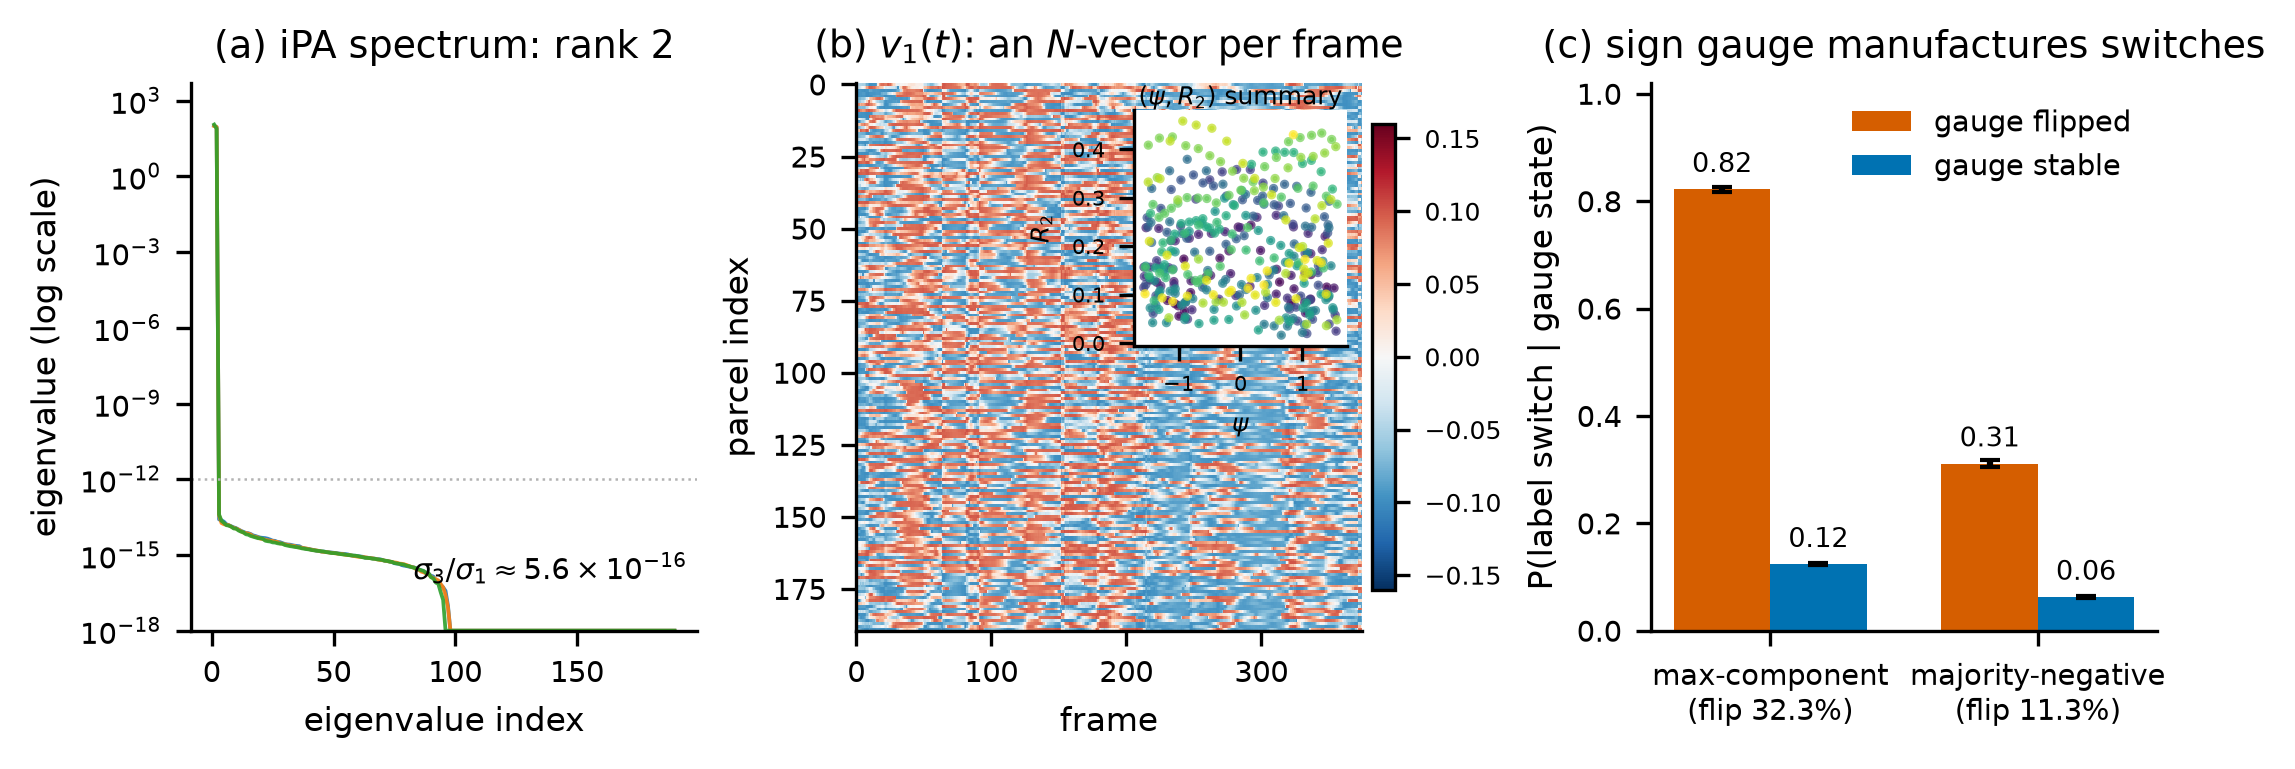
\includegraphics[width=\textwidth]{fig1_rank2_gauge.png}
\caption{Rank-2 structure and the sign gauge. (a) Eigenvalue spectrum of the iPA
matrix for three frames; two non-zero eigenvalues, $\sigma_3/\sigma_1\approx
5.6\times10^{-16}$. (b) The leading eigenvector across frames (continuity-aligned for
display): an $N=190$ vector per frame; the inset shows the two-parameter summary
$(\psi,R_2)$. (c) Probability of a label switch given a gauge flip vs no flip, for the
max-component and majority-negative conventions (HBN resting-state, $n=180$;
mean $\pm$ SEM).}
\label{fig:rank2}
\end{figure}

\subsection{The sign gauge is not benign}
In the 180-subject HBN resting-state sample, the max-absolute-component gauge flipped on
$32.3\%$ of frames and the majority-negative gauge on $11.3\%$. Under the max-component
gauge, a label switch followed a gauge flip with probability $0.822$, versus $0.124$
when the gauge did not flip; under the majority-negative gauge the corresponding
probabilities were $0.311$ and $0.063$. A projective $k$-means partition removes the
gauge; in that partition a previously reported second-order label statistic collapses
from $z=+138$ to $z\approx+0.5$ at $k=5$. The gauge therefore explains a large part of
the apparent ``state dynamics'' and must be fixed or quotiented out before any
label-based claim.

\subsection{The J-space spectral metrics collapse to occupancy}
Table \ref{tab:jspace} gives the J-space group contrasts; none is significant. The
$\bar J$ spectral metrics are occupancy-dominated: linear $R^2$ on the $k=3$ occupancy
is $0.556$ for $C_k$ and $0.657$ for $r_{\mathrm{eff}}$.
The quadratic $R^2$ is $0.766$ and $0.768$. The coupling
between the J-space metrics and the independent $k=5$ occupancy lens ($C_k$ partial
$r=-0.322$, $r_{\mathrm{eff}}=+0.340$) collapses after controlling the $k=3$ occupancy
to $+0.079$ ($p=0.175$) and $+0.023$ ($p=0.695$). This is the empirical form of
Corollary \ref{cor:noindependent}: the $\bar J$ operator is a re-encoding of the
occupancy.

\begin{table}[H]
\centering
\caption{Custom J-space group contrasts (switching-linear stay field, $N=307$).}
\begin{tabular}{lccc}
\toprule
Metric & $d$ & $p$ & spread \\
\midrule
Spectral concentration $C_k$ & $-0.085$ & $0.47$ & mean $0.817$, sd $0.011$ \\
Effective rank $r_{\mathrm{eff}}$ & $+0.083$ & $0.47$ & mean $6.29$, sd $0.07$ \\
\bottomrule
\end{tabular}
\label{tab:jspace}
\end{table}

\begin{figure}[H]
\centering
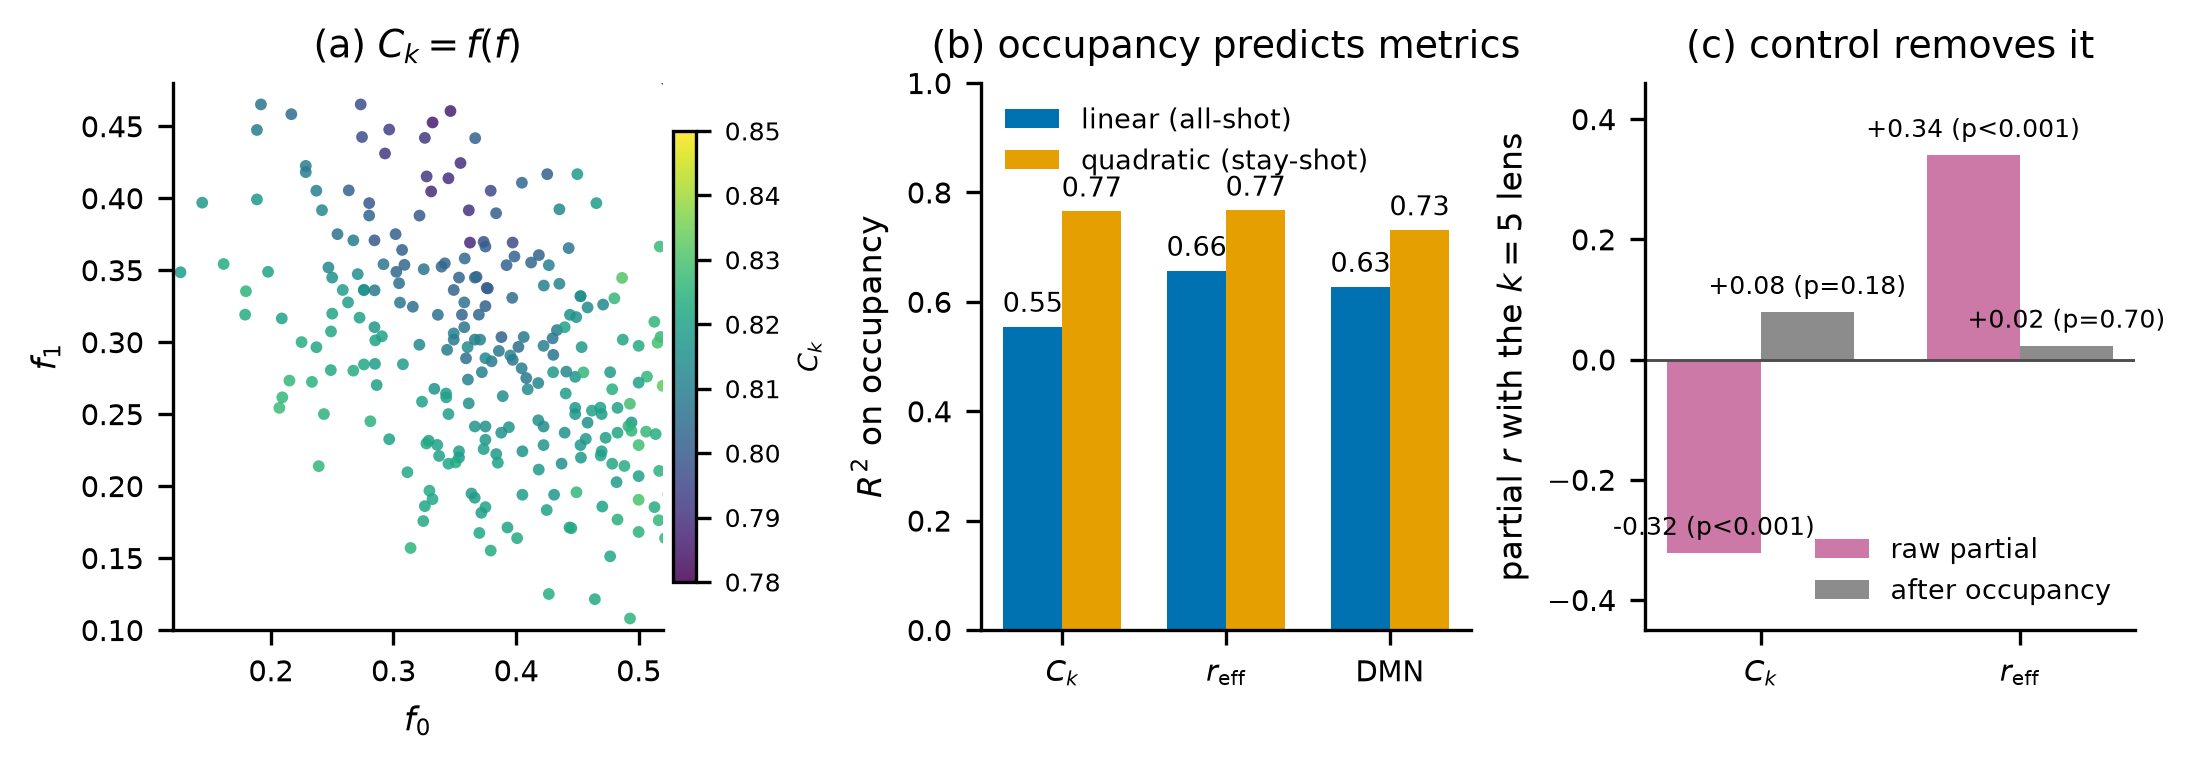
\includegraphics[width=\textwidth]{fig2_jspace_occupancy.png}
\caption{Occupancy degeneracy of the J-space. (a) The $k=3$ occupancy simplex, colored
by $C_k$; the metric is a function of $f$. (b) $R^2$ of each J-space metric on the
occupancy: linear (all-shot proxy) and quadratic (stay-shot proxy). (c) The coupling
between J-space metrics and the independent $k=5$ lens before and after controlling the
$k=3$ occupancy (partial $r$, $p$).}
\label{fig:jspace}
\end{figure}

\subsection{The pattern-defined effect is robust}
The $k=5$ de-novo lens gives a negative ADHD effect on the pattern-matched reduced state
(ADHD lower occupancy). Table \ref{tab:o2} reports the primary analysis. The fixed-effect
meta across the four site codes is $d=-0.302$ (parametric $p=0.00016$); the simple cohort
standardized difference is $d=-0.263$ ($p=0.00077$). The within-site-code permutation
gives $p=0.001$ (2,000-draw floor) and the FWER is $0.001$ (1,000-draw floor), with
$n=665$, $I^2=27.6\%$, and a random-effects estimate of $-0.294$ ($p=0.0029$).
Split-half reliability is $SB=0.586$ $[0.453,0.681]$, measured on the 220 subjects with
at least two runs; the single-run correlation is $r=0.415$. With true per-run motion
matching, the paired $d_z$ is $-0.172$ ($260$ pairs, $p=0.006$) and the matched
between-group $d$ is $-0.246$ [95\% CI $-0.428$ to $-0.074$]; a site+motion OLS gives
$b=-0.0162$ ($p=0.0020$, $n=640$). The effect is negative in three of the four site
codes; NeuroIMAGE reverses ($d=+0.115$, unadjusted $p=0.62$), which is disclosed as
site-code heterogeneity.

\begin{table}[H]
\centering
\caption{Pattern-matched LEiDA occupancy effect in ADHD-200 ($k=5$ de-novo lens).}
\begin{tabular}{lcc}
\toprule
Quantity & Value & Note \\
\midrule
$d$ (pattern-matched, FE meta) & $-0.302$ & 665 subjects (309 ADHD/356 TDC) \\
Simple cohort $d$ & $-0.263$ & $p=0.00077$ \\
Parametric $p$ & $0.00016$ & fixed-effect meta \\
Within-site-code permutation $p$ & $0.001$ & 2,000-draw floor \\
FWER & $0.001$ & 1,000-draw floor; max-$|d|$ over five states \\
$I^2$ & $27.6\%$ & random-effects $-0.294$ ($p=0.0029$) \\
Split-half $SB$ & $0.586$ $[0.453,0.681]$ & 220 two-run subjects; single-run $r=0.415$ \\
Motion-matched $d_z$ / $d$ & $-0.172$ / $-0.246$ & 260 pairs, $p=0.006$; CI $[-0.428,-0.074]$ \\
Site+motion $b$ & $-0.0162$ & $p=0.0020$ \\
Site-wise sign & $3/4$ negative & NeuroIMAGE $+0.115$ (unadjusted $p=0.62$) \\
\bottomrule
\end{tabular}
\label{tab:o2}
\end{table}

\begin{figure}[H]
\centering
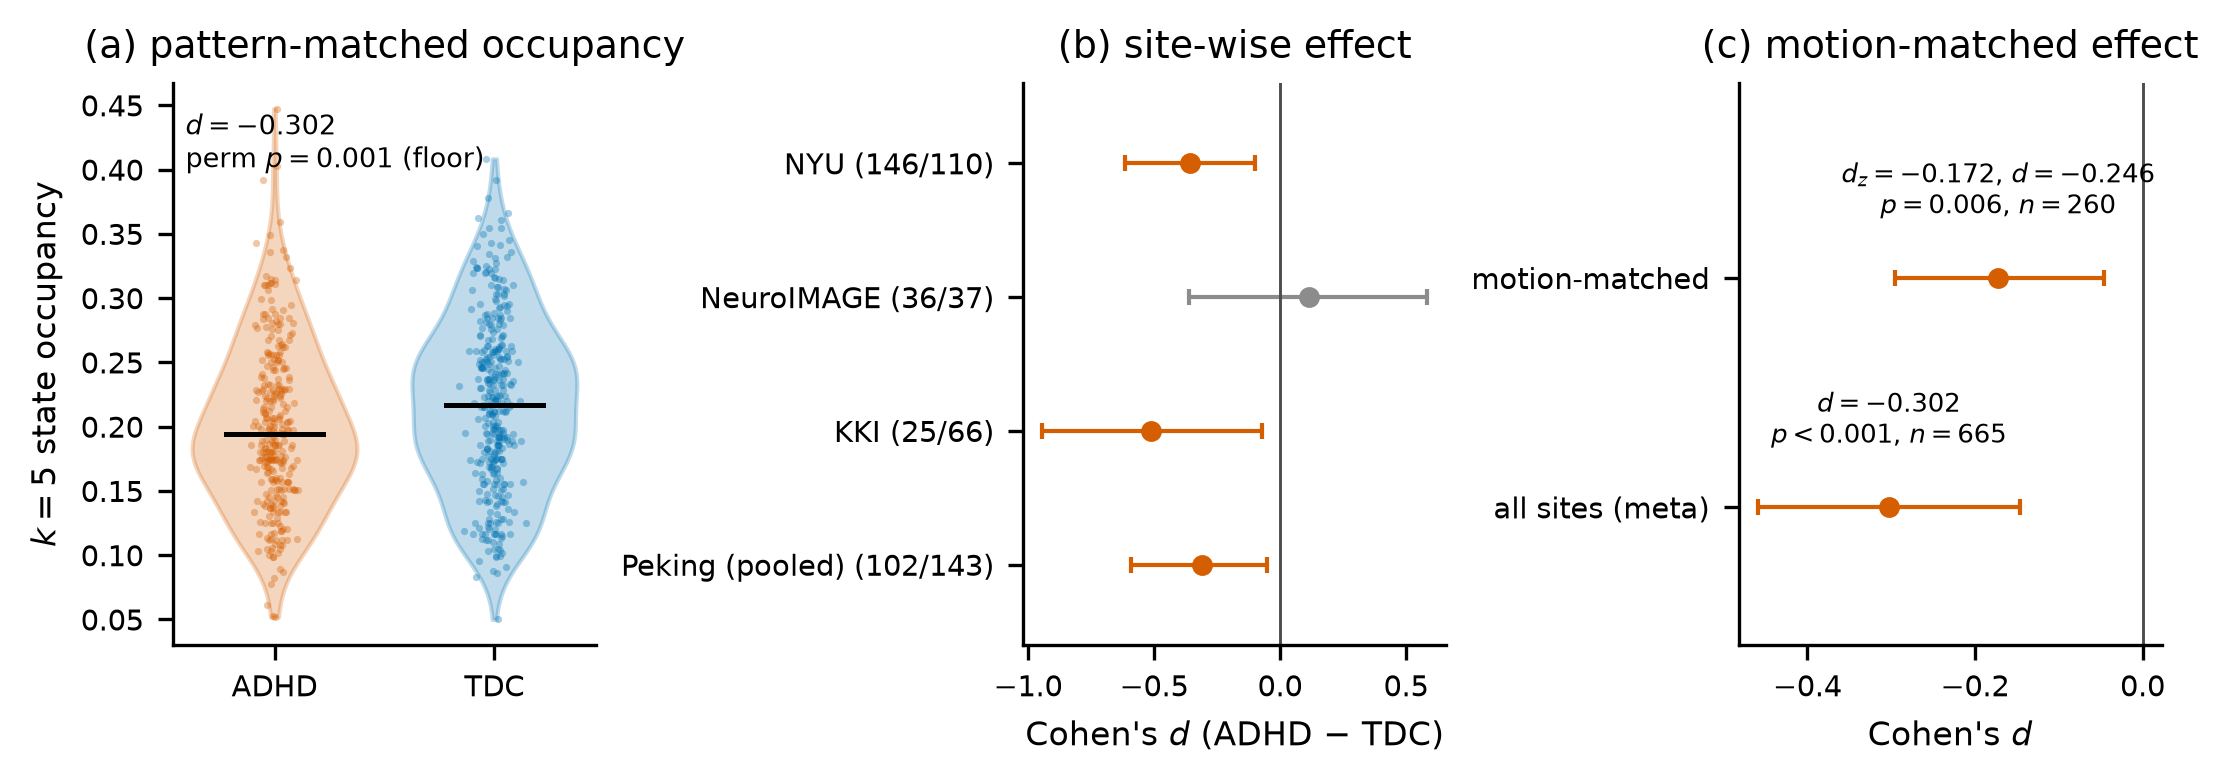
\includegraphics[width=\textwidth]{fig3_o2_effect.png}
\caption{Pattern-matched LEiDA occupancy effect in ADHD-200 ($k=5$ de-novo lens).
(a) Occupancy by group ($n=665$; 309 ADHD / 356 TDC). (b) Site-wise standardized
difference with bootstrap 95\% CI. (c) Meta-analytic effect and motion-matched paired
$d_z$ / between-group $d$ with 95\% CI.}
\label{fig:o2}
\end{figure}

\subsection{The pattern effect survives; the integer index does not}
Table \ref{tab:refit} reports the refit identifiability test. The literal index-4 effect
is $d=-0.0347$ ($50\%$ of refits negative, not significant). The pattern-matched effect
is $d=-0.2987$, with the 2.5--97.5th percentile of the 40 refit estimates at
$[-0.3645,-0.1915]$, and $100\%$ of refits negative. The index is recovered in
$9/40=22.5\%$ of refits, consistent with the $20\%$ chance level ($1/k$). The 40 refits share two-thirds of their data, so the nominal 95\%
interval $[11.8\%,37.1\%]$ overstates precision; the point estimate is consistent with
chance and cannot exclude recovery up to about $37\%$. The partition is
stable; the index is not. The correct claim is about ``a state'' identified by pattern,
not about ``state 4.''

\begin{table}[H]
\centering
\caption{Refit identifiability test (40 one-third-run refits; correlated subsamples).}
\begin{tabular}{lcc}
\toprule
Quantity & Value & Interpretation \\
\midrule
Literal index-4 $d$ & $-0.0347$ & null; 50\% refits negative \\
Pattern-matched $d$ & $-0.2987$ & 95\% CI $[-0.3645,-0.1915]$; 100\% negative \\
Index-4 recovery & $9/40=22.5\%$ & chance $20\%$; 95\% CI $11.8$--$37.1\%$ \\
\bottomrule
\end{tabular}
\label{tab:refit}
\end{table}

\begin{figure}[H]
\centering
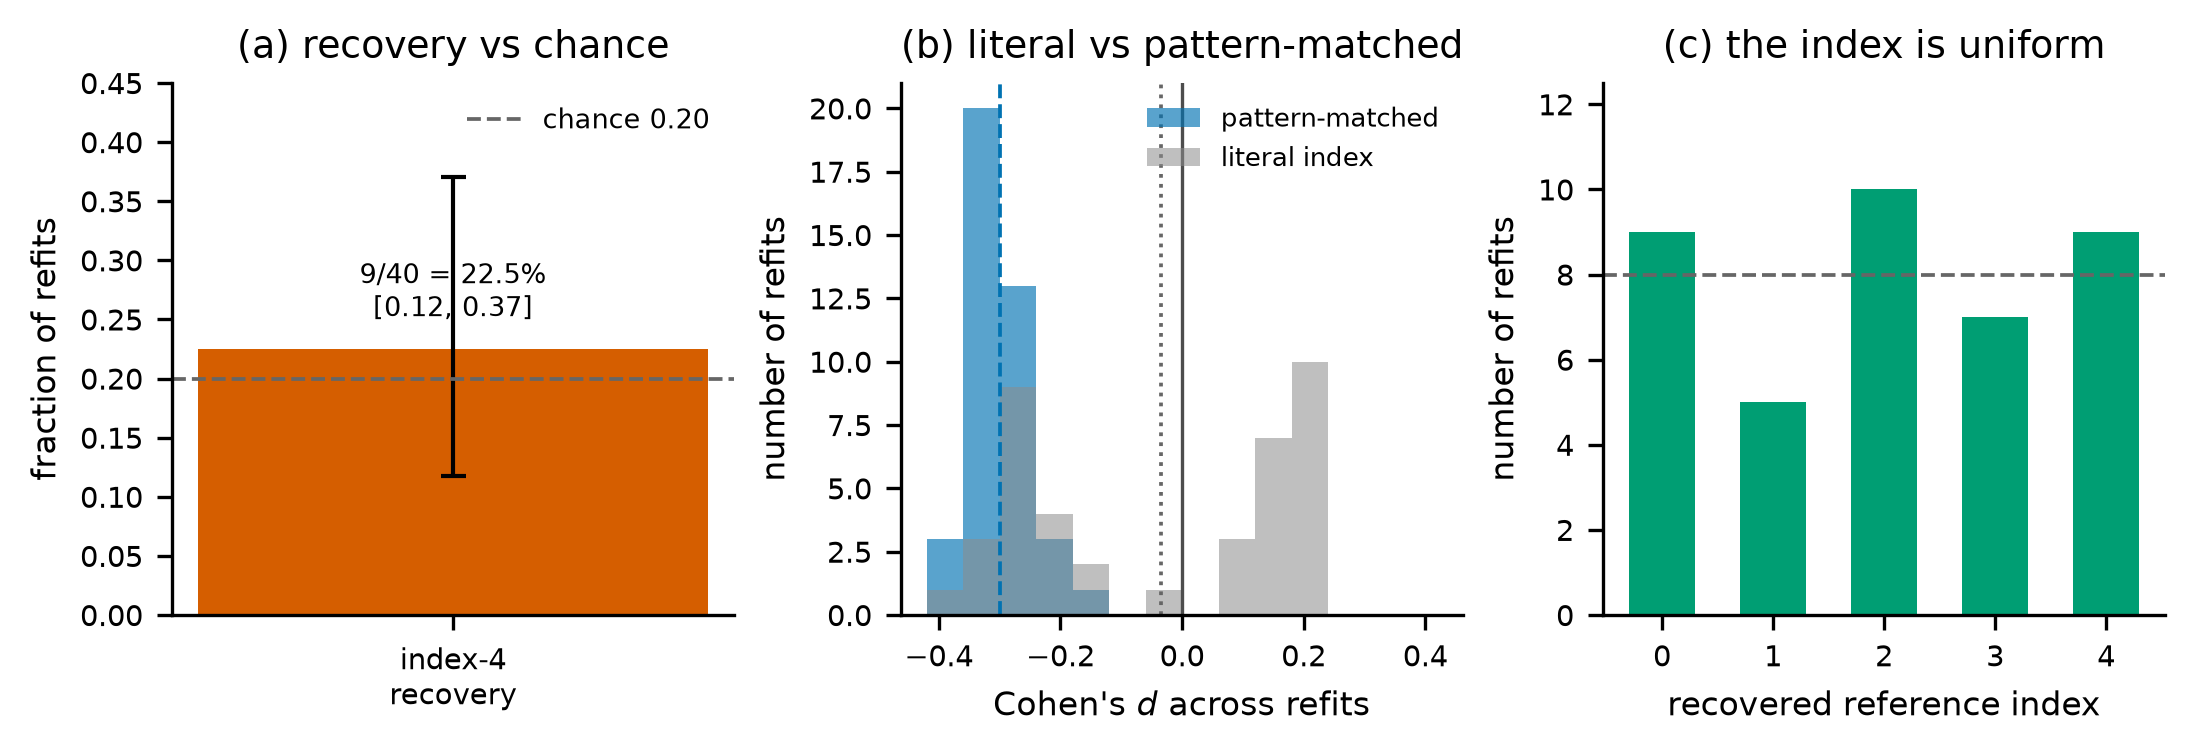
\includegraphics[width=\textwidth]{fig4_identifiability.png}
\caption{Named-state identifiability (40 one-third-run refits; correlated subsamples).
(a) Index-4 recovery vs the $1/k$ chance level (nominal 95\% CI). (b) Literal vs pattern-matched effect
sizes across refits. (c) Distribution of recovered indices vs the chance expectation.}
\label{fig:refit}
\end{figure}

The pattern itself---the centroid map and its network loadings---is not displayed
here; the effect is defined by that pattern (see Methods), not by a named index.

\begin{table}[H]
\centering
\caption{Prior dynamic-FC ADHD cohorts vs this reanalysis. Designs differ; direction only.}
\begin{tabular}{llll}
\toprule
Study & Operator / design & $n$ & Direction \\
\midrule
de Lacy 2019 & dynamic FNC, dwell/meta-state & 504 (252/252) & reduced DMN dwell \\
Shappell 2021 & sliding-window dFC & --- & hyperconnected states \\
Ahmadi 2021 & sliding-window dFC & --- & less time in one state \\
Kaboodvand 2020 & synergetic configurations & --- & altered configurations \\
This reanalysis & LEiDA occupancy (pattern-matched) & 665 & lower occupancy, $d=-0.302$ \\
\bottomrule
\end{tabular}
\label{tab:prior}
\end{table}

\subsection{Robustness}
The pattern effect survives within-site-code permutation, reliability gating, motion
matching, and site-wise analysis. It is not explained by age, sex, site, or motion, and
it is negative in three of the four site codes, with NeuroIMAGE reversing.
Gauge robustness beyond the max-component gauge used here---majority-negative and
projective partitions---is computed in code but not reported here; the named-index
result does not depend on which gauge fixes the labels.

\section{Discussion}
\label{sec:discussion}

The LEiDA state is a projective leading eigenvector: an $N$-dimensional pattern. The iPA
matrix is rank 2, but that does not make the state two numbers; it makes the spectral
subspace two-dimensional. The state becomes a two-number object only when one adopts
the occupancy of a learned operator, and even then the two numbers are the $k-1$ simplex
coordinates of the J-space, not the leading eigenvector. This distinction is the
difference between a mathematical fact about a matrix and a false claim about a brain
state.

The J-space is useful as a coordinate system, but its stay-field summaries are functions
of occupancy (Remark \ref{thm:occupancy}). A J-space mean difference is therefore an
occupancy difference in operator coordinates. The coupling between the J-space metrics
and the independent $k=5$ lens is cross-lens occupancy consistency, not a mechanism. A
future J-space claim should target an order-sensitive object that escapes the
theorem---a fitted transition matrix, a lagged commutator, or a time-varying operator;
the present static shared-operator field cannot supply one.

ADHD shows lower pattern-matched occupancy at the group level. The literal index is
null, so the claim is about a pattern-defined state, not an integer index. Overlap with
de Lacy and Calhoun makes this a reanalysis; the contribution is the identifiability
result, not discovery of the effect.

Rank-2 and sign ambiguity are prior art \cite{Glerean2012,Olsen2022,EiDA2024}; the
switching-linear class is prior art \cite{Linderman2017,Taghia2018}. New here: the
occupancy-degeneracy remark, the $1/k$ identifiability baseline, and the pattern-defined
effect under an exact null.

\subsection*{Constraints that shaped the finding}

The occupancy test is limited by what public ADHD data can support. ADHD-200 is the only
cohort available here that combines a categorical ADHD diagnosis with an $N$ large enough to
test the pattern effect at the required reliability; that is why the test is there and
not in an independent cohort. The other public cohorts are limited in different ways.
HBN provides the largest pediatric sample but its categorical diagnosis is behind a data
use agreement; the open release carries bifactor scores only. ds005899 has $26$ ADHD and
$35$ comparison children on a five-minute scan. ds000030 has $42$ ADHD adults on a
different protocol and atlas. PennLEAD is a single site with 27 unique ADHD subjects
(group sizes 41/45 in the n-back subset and 42/45 in the rest subset). These cohorts are
not interchangeable with ADHD-200 for the present test, and
their limitations are why the finding is a single-cohort pattern-defined reanalysis
rather than an independent replication.

At $n=665$, the 80% power threshold for a
two-group difference is $d\approx0.22$; the data are adequate to detect the moderate
effect reported here and a large effect ($d\approx0.66$), but not a small effect
($d\approx0.18$) at the measured reliability. The binding constraints are the absence of
a second categorical-diagnosis cohort, the split-half reliability ($SB=0.586$ on 220
two-run subjects; single-run $r=0.415$; attenuation-corrected effect $d\approx0.39$--$0.47$),
the $70.5\%$ overlap with the ADHD-200 sample of de Lacy and Calhoun \cite{deLacy2019},
and the one reversing site code.

The J-space model is trained in-sample, so per-subject
J-space estimates are bounded by the in-sample fit.
The per-subject operator is not identifiable at $T\approx355$, and the SVD metrics are
not invariant under non-orthogonal latent reparameterization; the J-space summaries
should be read as population-level descriptions, not stable subject properties. The refit identifiability test uses one-third-run
subsamples; full-data refits and a second lens are needed to generalize the $22.5\%$
estimate. The chance model assumes exchangeable labels, which is a null, not a
description of the data.

These constraints do not weaken the two claims the paper actually makes: the J-space is
an occupancy re-encoding, and the named state index is not identifiable. They do bound
the empirical claim: the pattern effect is a group-level, single-cohort, pattern-defined
difference, not an individual biomarker and not a named-state effect.

\subsection*{What would change the conclusion}

Three tests would materially change the picture. A continuous-state test on
$(\psi,R_2)$ or on the projective class with an exact null would avoid the named index
entirely and show whether the pattern effect survives without a $k$-means partition. The
refit identifiability test in a second lens and a second cohort would show whether the
$1/k$ result is a property of this pipeline or of the state definition. A time-varying
operator would show whether the J-space can escape the occupancy degeneracy; the present
static shared-operator field cannot.

\section{Conclusion}
\label{sec:conclusion}

We separated three objects that are often conflated: the rank-2 phase-alignment matrix,
the learned Jacobian operator, and the named $k$-means state. The first is a
two-dimensional spectral object but has an $N$-dimensional eigenvector; the second is a
shared-operator occupancy mixture whose stay-field summaries are functions of $k-1=2$
numbers; the third is not identifiable, with index recovery at $1/k$ chance. Applying
the framework to ADHD-200, we found a negative, motion-robust, pattern-matched occupancy
effect (ADHD lower occupancy; $d=-0.302$, permutation $p=0.001$ [2,000-draw floor], FWER
$0.001$ [1,000-draw floor], $n=665$, $SB=0.586$) and a null literal index effect
($d=-0.035$), with $22.5\%$ index recovery versus $20\%$ chance. The effect is real in
this cohort; the named state is not. Dynamic-FC claims about ``state
$s$'' should therefore report a refit identifiability test and a pattern-matched effect,
or be stated as claims about ``some state.''

\section*{Data and Code Availability}
Data are ADHD-200 and HBN fMRI as described in Data and Methods; code to reproduce
all numbers is available in the accompanying repository.

\begin{thebibliography}{99}

\bibitem{Cabral2017}
Cabral J, Vidaurre D, Marques P, Magalh\~aes R, Silva Moreira P, Miguel Soares J, Deco G,
Sousa N, Kringelbach ML.
Cognitive performance in healthy older adults relates to spontaneous switching between
states of functional connectivity during rest.
\textit{Scientific Reports}. 2017;7:5135. doi:10.1038/s41598-017-05425-7.

\bibitem{Glerean2012}
Glerean E, Salmi J, Lahnakoski JM, J\"a\"askel\"ainen IP, Sams M.
Functional magnetic resonance imaging phase synchronization as a measure of dynamic
functional connectivity.
\textit{Brain Connectivity}. 2012;2(2):91--101. doi:10.1089/brain.2011.0068.

\bibitem{Olsen2022}
Olsen AS, Lykkebo-Vall\o e A, Ozenne B, Madsen MK, Stenb\ae k DS, Armand S, M\o rup M, Ganz
M, Knudsen GM, Fisher PM.
Psilocybin modulation of time-varying functional connectivity is associated with plasma
psilocin and subjective effects.
\textit{NeuroImage}. 2022;264:119716. doi:10.1016/j.neuroimage.2022.119716.

\bibitem{EiDA2024}
de Alteriis G, MacNicol E, Hancock F, Ciaramella A, Cash D, Expert P, Turkheimer FE.
EiDA: A lossless approach for dynamic functional connectivity; application to fMRI data of
a model of ageing.
\textit{Imaging Neuroscience}. 2024;2:1--22. doi:10.1162/imag_a_00113.

\bibitem{Chen2018}
Chen RTQ, Rubanova Y, Bettencourt J, Duvenaud DK.
Neural ordinary differential equations.
In: \textit{Advances in Neural Information Processing Systems (NeurIPS)}. 2018;31.

\bibitem{Linderman2017}
Linderman S, Johnson M, Miller A, Adams R, Blei D, Paninski L.
Bayesian learning and inference in recurrent switching linear dynamical systems.
In: \textit{Proceedings of the 20th International Conference on Artificial Intelligence and
Statistics (AISTATS)}. PMLR 54:914--922, 2017.

\bibitem{Taghia2018}
Taghia J, Cai W, Ryali S, Kochalka J, Nicholas J, Chen T, Menon V.
Uncovering hidden brain state dynamics that regulate performance and decision-making during
cognition.
\textit{Nature Communications}. 2018;9:2505. doi:10.1038/s41467-018-04723-6.

\bibitem{Tang2026}
Tang J, Wang Y, Xu X, Pan X, Wang R.
Reorganization of global phase pattern in complex brain network during aging revealed by
leading eigenvector dynamics analysis.
\textit{International Journal of Bifurcation and Chaos}. 2026;36(8):2650106.
doi:10.1142/S0218127426501063.

\bibitem{ADHD2002012}
The ADHD-200 Consortium.
The ADHD-200 Consortium: a model to advance the translational potential of neuroimaging in
clinical neuroscience.
\textit{Frontiers in Systems Neuroscience}. 2012;6:62. doi:10.3389/fnsys.2012.00062.

\bibitem{deLacy2019}
de Lacy N, Calhoun VD.
Dynamic connectivity and the effects of maturation in youth with attention deficit
hyperactivity disorder.
\textit{Network Neuroscience}. 2019;3(1):195--216. doi:10.1162/netn_a_00063.

\bibitem{Shappell2021}
Shappell HM, Duffy KA, Rosch KS, Pekar JJ, Mostofsky SH, Lindquist MA, Cohen JR.
Children with attention-deficit/hyperactivity disorder spend more time in hyperconnected
network states and less time in segregated network states as revealed by dynamic
connectivity analysis.
\textit{NeuroImage}. 2021;229:117753. doi:10.1016/j.neuroimage.2021.117753.

\bibitem{Ahmadi2021}
Ahmadi M, Kazemi K, Ku\'c K, Cybulska-Klosowicz A, Helfroush MS, Aarabi A.
Resting state dynamic functional connectivity in children with attention
deficit/hyperactivity disorder.
\textit{Journal of Neural Engineering}. 2021;18(4):0460d1.
doi:10.1088/1741-2552/ac16b3.

\bibitem{Kaboodvand2020}
Kaboodvand N, Iravani B, Fransson P.
Dynamic synergetic configurations of resting-state networks in ADHD.
\textit{NeuroImage}. 2020;207:116347. doi:10.1016/j.neuroimage.2019.116347.

\bibitem{Hennig2007}
Hennig C.
Cluster-wise assessment of cluster stability.
\textit{Computational Statistics \& Data Analysis}. 2007;52(1):258--271.
doi:10.1016/j.csda.2006.11.025.

\bibitem{vonLuxburg2010}
von Luxburg U.
Clustering stability: an overview.
\textit{Foundations and Trends in Machine Learning}. 2010;2(3):235--274.
doi:10.1561/2200000008.

\bibitem{Stephens2000}
Stephens M.
Dealing with label switching in mixture models.
\textit{Journal of the Royal Statistical Society: Series B}. 2000;62(4):795--809.
doi:10.1111/1467-9868.00265.

\bibitem{Jasra2005}
Jasra A, Holmes CC, Stephens DA.
Markov chain Monte Carlo methods and the label switching problem in Bayesian mixture
modeling.
\textit{Statistical Science}. 2005;20(1):50--67. doi:10.1214/088342305000000016.

\end{thebibliography}

\end{document}
